% include the figures path relative to the master file
\graphicspath{ {./content/method/figures/} }

\section{\uppercase{Balancing strategies}}\label{sec:met}

\noindent Considering a binary classification problem, the class with the smallest number of samples is defined as the \textit{minority} class and its counterpart is defined as the \textit{majority} class.
The problem of data balancing corresponds to equalizing the number of samples of both the minority and majority classes. This task can be achieved in either data or feature space.

\subsection{Data space sampling}

Data space sampling is related with the generation of new synthetic samples by modifying the original data ahead of any feature extraction processes.
\Ac{os} is performed on the original dataset by generating synthetic melanoma images based on two types of deformation~\cite{rastgoo2015ensemble}. Furthermore, cubic b-spline interpolation is used with both methods to approximate non-integer points in the image.
 
\begin{description}
	\item[\Ac{rdgm}] achieved by deforming the original image by adding a random Gaussian motion $\mathcal{N}(\mu, \sigma) = (5,5)$ at each pixel compounded with a global rotation of~\SI{80}{\degree}.
	\item[\Ac{bd}] corresponds to a deformation of the original image using barrel distortion compounded with a global rotation of~\SI{145}{\degree}.
\end{description}

A synthetic example illustrating the results of these deformation is presented in Fig.\,\ref{fig:DSOS}.

% \begin{table*}
% \caption{The obtained results with different balancing techniques for color and texture features using a \acs*{rf} classifier. The first and second highest results for each feature set are highlighted in dark and lighter gray colors respectively.}
% \centering
% \resizebox{1.\textwidth}{!}{ \begin{tabular}{l cccccc		cccccc		cccccc}
\toprule
Features &  \multicolumn{6}{l}{Color}& \multicolumn{6}{l}{Texture} & \multicolumn{6}{l}{Combined}\\
  \cmidrule(r){2-7}  \cmidrule(r){8-13}  \cmidrule(r){14-19}  
		   & \multicolumn{2}{c}{$C_{1}$}& \multicolumn{2}{c}{$C_{2}$}& \multicolumn{2}{c}{$C_{1,2}$}& \multicolumn{2}{c}{$T_{1}$} &  \multicolumn{2}{c}{$T_{2}$} & \multicolumn{2}{c}{$T_{1,2}$}& \multicolumn{2}{c}{$T_{1},C_{1,2}$}& \multicolumn{2}{c}{$T_{2},C_{1,2}$}& \multicolumn{2}{c}{$T_{1,2},C_{1,2}$}\\ 
  \cmidrule(r){2-3}  \cmidrule(r){4-5} \cmidrule(r){6-7} \cmidrule(r){8-9} \cmidrule(r){10-11} \cmidrule(r){12-13} \cmidrule(r){14-15} \cmidrule(r){16-17} \cmidrule(r){18-19} 
  Balancing techniques & \makebox[0.5cm][l]{\acs*{se}}& \makebox[0.5cm][l]{\acs*{sp}} & \makebox[0.5cm][l]{\acs*{se}} & \makebox[0.5cm][l]{\acs*{sp}} & \makebox[0.5cm][l]{\acs*{se}} &\makebox[0.5cm][l]{\acs*{sp}} &\makebox[0.5cm][l]{\acs*{se}} &\makebox[0.5cm][l]{\acs*{sp}} &\makebox[0.5cm][l]{\acs*{se}} & \makebox[0.5cm][l]{\acs*{sp}} &\makebox[0.5cm][l]{\acs*{se}} &\makebox[0.5cm][l]{\acs*{sp}} & \makebox[0.5cm][l]{\acs*{se}} &\makebox[0.5cm][l]{\acs*{sp}} &\makebox[0.5cm][l]{\acs*{se}} &\makebox[0.5cm][l]{\acs*{sp}}& \makebox[0.5cm][l]{\acs*{se}} &\makebox[0.5cm][l]{\acs*{sp}}  \\ \midrule
\multicolumn{1}{c}{IB} & 52.50 & 89.58 & 75.00 & 88.75 & 71.25& 87.50& 38.75 & 91.67 & 60.00 & 96.25 & 66.25 & 93.75 &73.75 & 89.58&71.25 & 89.58 & 71.25& 92.50\\
\midrule \midrule
\multicolumn{1}{c}{\acs*{os}} &\cellcolor[gray]{0.6}93.75 &\cellcolor[gray]{0.6}66.67 &80.00 & 86.25& 82.50 & 87.08  & 43.75 &83.75 &72.50& 90.00 & 70.00& 91.67  &77.50 & 87.08 &81.25 &88.33 &78.75 &88.33  \\
\midrule \midrule
\multicolumn{1}{c}{\acs*{ros}} &55.00 & 80.83& 80.00 & 84.17& 72.50 &85.42 &42.50 & 82.08 &60.00 & 89.17 &66.25 &87.92&75.00&85.42&73.75&86.25&73.75 &85.83\\
\multicolumn{1}{c}{\acs*{smote}} & 60.00 & 82.50 & 78.75 & 84.58 & 75.00 & 70.00 & 56.25 & 74.17 & 61.25 & 87.50 & 84.17 &87.08 & 78.75& 85.00 &73.75 & 84.58 &73.75&85.00 \\ 
\midrule
\multicolumn{1}{c}{\ac{rus}} & 72.50 & 72.92 & 86.25 & 80.00 & 78.75 &80.00 & 67.50 & 53.33 &76.25 &76.25  &85.00 &78.75 &\cellcolor[gray]{0.6}91.25 & \cellcolor[gray]{0.6}75.00 & 85.00 & 78.75 &\cellcolor[gray]{0.6}92.50 &\cellcolor[gray]{0.6}78.33\\
\multicolumn{1}{c}{\acs*{tl}} & 51.25 & 86.25 & 76.25 & 87.92&67.50 & 88.33  & 37.50 & 87.92 & 65.00 &90.42 & 68.75 & 91.67 & 73.75 & 88.75 &63.75 & 90.00 & 72.50 & 91.25\\
\multicolumn{1}{c}{\acs*{cus}} & 81.25 & 67.92 & 80.00 & 84.58&\cellcolor[gray]{0.8} 86.25 & \cellcolor[gray]{0.8}80.42 & 56.25 & 65.83 & 70.00 & 77.50 & 85.00 & 77.08 & 83.75 & 81.25 & 80.00 & 84.17 & 83.75 & 82.92\\
\multicolumn{1}{c}{\acs*{nm1}} & 67.50 & 72.08 & 86.25 & 79.17& 85.00 & 82.50 & 72.50 & 43.75 & 80.00 & 62.50 &\cellcolor[gray]{0.6} 87.50 &\cellcolor[gray]{0.6} 66.67 & 85.00 & 82.08 & \cellcolor[gray]{0.8}86.25 &\cellcolor[gray]{0.8}80.42 & 87.50 & 80.83\\
\multicolumn{1}{c}{\acs*{nm2}} & 70.00 & 72.92 & 86.25 & 81.25 & 85.00 & 82.92 & \cellcolor[gray]{0.8}76.25 &\cellcolor[gray]{0.8} 48.75& \cellcolor[gray]{0.6}86.25 &\cellcolor[gray]{0.6} 40.83 & \cellcolor[gray]{0.8}86.25 &\cellcolor[gray]{0.8} 51.25& \cellcolor[gray]{0.8}87.50 & \cellcolor[gray]{0.8}82.08 &\cellcolor[gray]{0.6}92.50 &\cellcolor[gray]{0.6}77.50& \cellcolor[gray]{0.8}91.25 &\cellcolor[gray]{0.8}81.67\\
\multicolumn{1}{c}{\acs*{nm3}} & \cellcolor[gray]{0.8}82.50 & \cellcolor[gray]{0.8}75.00 &\cellcolor[gray]{0.8} 87.50 &\cellcolor[gray]{0.8} 80.83 & 85.00 & 80.42 &73.75 & 55.83 & 72.50 & 82.50 & 82.50 & 80.42 & 83.75 & 81.25 & 85.00 & 80.00 & 86.25 & 80.42\\
\multicolumn{1}{c}{\ac{ncr}} & {\color{blue}66.25} & {\color{blue}76.67} & \cellcolor[gray]{0.6}{\color{blue} 87.50} &\cellcolor[gray]{0.6}{\color{blue} 81.25} &{\color{blue}85.00} &{\color{blue} 82.08} & {\color{blue}67.50} & {\color{blue}67.92} & {\color{blue}75.00} & {\color{blue}85.83} & {\color{blue} 82.50} & {\color{blue} 83.33} & {\color{blue} 86.25} & {\color{blue} 81.67} & {\color{blue}82.50} &{\color{blue} 85.00} & {\color{blue}83.75} &{\color{blue} 85.42}\\
\midrule
\multicolumn{1}{c}{\acs*{smote} + \acs*{enn}} & 76.25 & 73.33 & 85.00 & 81.25 & 85.00 & 82.08 &\cellcolor[gray]{0.6} 81.25 &\cellcolor[gray]{0.6} 56.25 & 76.25 & 82.08 & 80.00 & 79.58 & 86.25 & 81.25 & 83.75 & 82.50 & 78.75 & 82.92\\
\multicolumn{1}{c}{\acs*{smote} + \acs*{tl}} & 75.00 & 73.75 & 83.75 & 82.50 & \cellcolor[gray]{0.6}87.50 &\cellcolor[gray]{0.6}80.83 & 72.50 & 59.17 & \cellcolor[gray]{0.8}77.50 &\cellcolor[gray]{0.8} 82.08 & 78.75 & 78.75 & 85.00 & 82.08 & 77.50 & 82.92 & 88.75 & 82.50\\
\bottomrule
\end{tabular}
}
% \label{tab:tab1}
% \end{table*}

\newpage

\onecolumn

\begin{landscape}

\begin{figure*}[Ht]
  \centering
  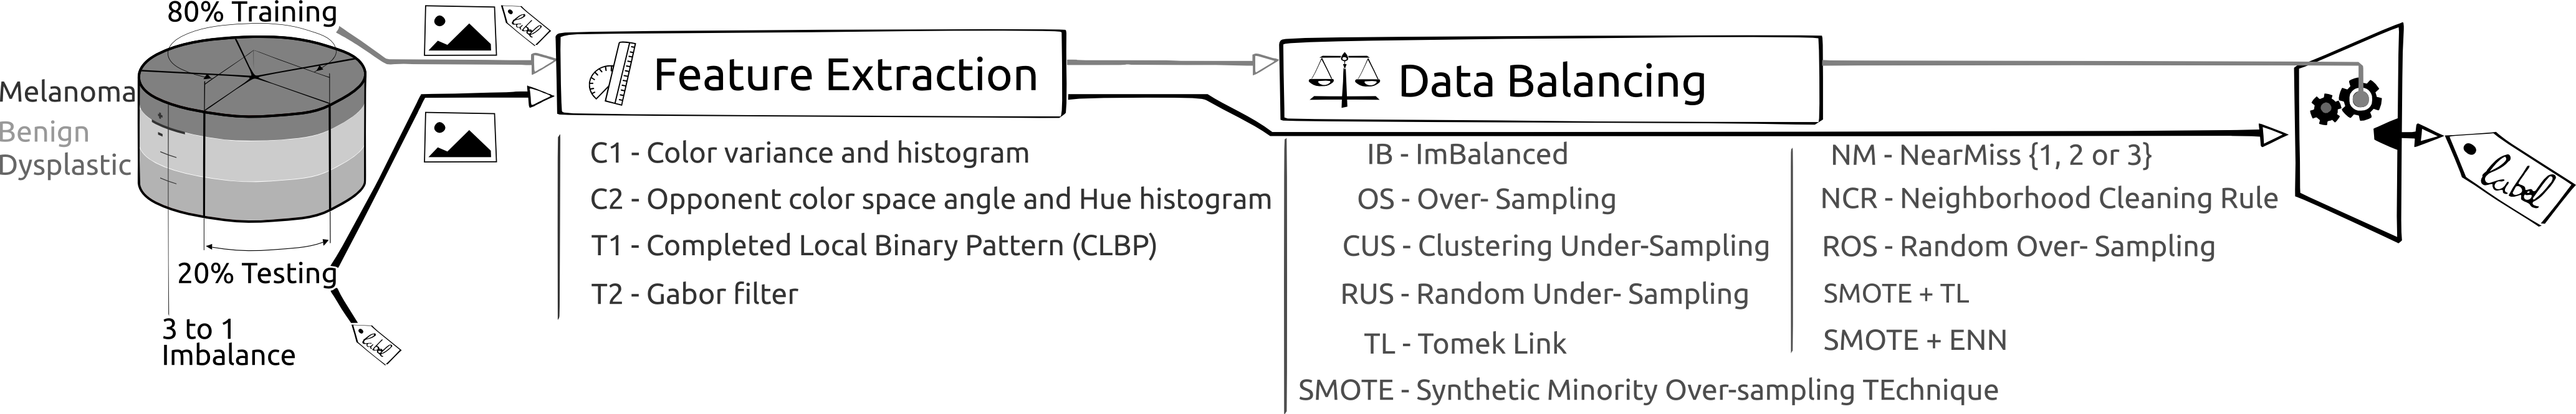
\includegraphics[width=1.4\textwidth]{method.png}
  \caption{Framework outline}
	\label{fig:schema}
\end{figure*}

\begin{table*}
\caption{The obtained results with different balancing techniques for color and texture features using a \acs*{rf} classifier. The first and second highest results for each feature set are highlighted in dark and lighter gray colors, respectively.}
\centering
\resizebox{1.42\textwidth}{!}{
\begin{tabular}{l cccccc		cccccc		cccccc}
\toprule
Features &  \multicolumn{6}{l}{Color}& \multicolumn{6}{l}{Texture} & \multicolumn{6}{l}{Combined}\\
  \cmidrule(r){2-7}  \cmidrule(r){8-13}  \cmidrule(r){14-19}  
		   & \multicolumn{2}{c}{$C_{1}$}& \multicolumn{2}{c}{$C_{2}$}& \multicolumn{2}{c}{$C_{1,2}$}& \multicolumn{2}{c}{$T_{1}$} &  \multicolumn{2}{c}{$T_{2}$} & \multicolumn{2}{c}{$T_{1,2}$}& \multicolumn{2}{c}{$T_{1},C_{1,2}$}& \multicolumn{2}{c}{$T_{2},C_{1,2}$}& \multicolumn{2}{c}{$T_{1,2},C_{1,2}$}\\ 
  \cmidrule(r){2-3}  \cmidrule(r){4-5} \cmidrule(r){6-7} \cmidrule(r){8-9} \cmidrule(r){10-11} \cmidrule(r){12-13} \cmidrule(r){14-15} \cmidrule(r){16-17} \cmidrule(r){18-19} 
  Balancing techniques & \makebox[0.5cm][l]{\acs*{se}}& \makebox[0.5cm][l]{\acs*{sp}} & \makebox[0.5cm][l]{\acs*{se}} & \makebox[0.5cm][l]{\acs*{sp}} & \makebox[0.5cm][l]{\acs*{se}} &\makebox[0.5cm][l]{\acs*{sp}} &\makebox[0.5cm][l]{\acs*{se}} &\makebox[0.5cm][l]{\acs*{sp}} &\makebox[0.5cm][l]{\acs*{se}} & \makebox[0.5cm][l]{\acs*{sp}} &\makebox[0.5cm][l]{\acs*{se}} &\makebox[0.5cm][l]{\acs*{sp}} & \makebox[0.5cm][l]{\acs*{se}} &\makebox[0.5cm][l]{\acs*{sp}} &\makebox[0.5cm][l]{\acs*{se}} &\makebox[0.5cm][l]{\acs*{sp}}& \makebox[0.5cm][l]{\acs*{se}} &\makebox[0.5cm][l]{\acs*{sp}}  \\ \midrule
\multicolumn{1}{c}{IB} & 52.50 & 89.58 & 75.00 & 88.75 & 71.25& 87.50& 38.75 & 91.67 & 60.00 & 96.25 & 66.25 & 93.75 &73.75 & 89.58&71.25 & 89.58 & 71.25& 92.50\\
\midrule \midrule
\multicolumn{1}{c}{\acs*{os}} &\cellcolor[gray]{0.6}93.75 &\cellcolor[gray]{0.6}66.67 &80.00 & 86.25& 82.50 & 87.08  & 43.75 &83.75 &72.50& 90.00 & 70.00& 91.67  &77.50 & 87.08 &81.25 &88.33 &78.75 &88.33  \\
\midrule \midrule
\multicolumn{1}{c}{\acs*{ros}} &55.00 & 80.83& 80.00 & 84.17& 72.50 &85.42 &42.50 & 82.08 &60.00 & 89.17 &66.25 &87.92&75.00&85.42&73.75&86.25&73.75 &85.83\\
\multicolumn{1}{c}{\acs*{smote}} & 60.00 & 82.50 & 78.75 & 84.58 & 75.00 & 70.00 & 56.25 & 74.17 & 61.25 & 87.50 & 84.17 &87.08 & 78.75& 85.00 &73.75 & 84.58 &73.75&85.00 \\ 
\hdashline \noalign{\vskip 3pt}
\multicolumn{1}{c}{\acs*{rus}} & 72.50 & 72.92 & 86.25 & 80.00 & 78.75 &80.00 & 67.50 & 53.33 &76.25 &76.25  &85.00 &78.75 &\cellcolor[gray]{0.6}91.25 & \cellcolor[gray]{0.6}75.00 & 85.00 & 78.75 &\cellcolor[gray]{0.6}92.50 &\cellcolor[gray]{0.6}78.33\\
\multicolumn{1}{c}{\acs*{tl}} & 51.25 & 86.25 & 76.25 & 87.92&67.50 & 88.33  & 37.50 & 87.92 & 65.00 &90.42 & 68.75 & 91.67 & 73.75 & 88.75 &63.75 & 90.00 & 72.50 & 91.25\\
\multicolumn{1}{c}{\acs*{cus}} & 81.25 & 67.92 & 80.00 & 84.58&\cellcolor[gray]{0.8} 86.25 & \cellcolor[gray]{0.8}80.42 & 56.25 & 65.83 & 70.00 & 77.50 & 85.00 & 77.08 & 83.75 & 81.25 & 80.00 & 84.17 & 83.75 & 82.92\\
\multicolumn{1}{c}{\acs*{nm1}} & 67.50 & 72.08 & 86.25 & 79.17& 85.00 & 82.50 & 72.50 & 43.75 & 80.00 & 62.50 &\cellcolor[gray]{0.6} 87.50 &\cellcolor[gray]{0.6} 66.67 & 85.00 & 82.08 & \cellcolor[gray]{0.8}86.25 &\cellcolor[gray]{0.8}80.42 & 87.50 & 80.83\\
\multicolumn{1}{c}{\acs*{nm2}} & 70.00 & 72.92 & 86.25 & 81.25 & 85.00 & 82.92 & \cellcolor[gray]{0.8}76.25 &\cellcolor[gray]{0.8} 48.75& \cellcolor[gray]{0.6}86.25 &\cellcolor[gray]{0.6} 40.83 & \cellcolor[gray]{0.8}86.25 &\cellcolor[gray]{0.8} 51.25& \cellcolor[gray]{0.8}87.50 & \cellcolor[gray]{0.8}82.08 &\cellcolor[gray]{0.6}92.50 &\cellcolor[gray]{0.6}77.50& \cellcolor[gray]{0.8}91.25 &\cellcolor[gray]{0.8}81.67\\
\multicolumn{1}{c}{\acs*{nm3}} & \cellcolor[gray]{0.8}82.50 & \cellcolor[gray]{0.8}75.00 &\cellcolor[gray]{0.8} 87.50 &\cellcolor[gray]{0.8} 80.83 & 85.00 & 80.42 &73.75 & 55.83 & 72.50 & 82.50 & 82.50 & 80.42 & 83.75 & 81.25 & 85.00 & 80.00 & 86.25 & 80.42\\
\multicolumn{1}{c}{\acs*{ncr}} & {\color{blue}66.25} & {\color{blue}76.67} & \cellcolor[gray]{0.6}{\color{blue} 87.50} &\cellcolor[gray]{0.6}{\color{blue} 81.25} &{\color{blue}85.00} &{\color{blue} 82.08} & {\color{blue}67.50} & {\color{blue}67.92} & {\color{blue}75.00} & {\color{blue}85.83} & {\color{blue} 82.50} & {\color{blue} 83.33} & {\color{blue} 86.25} & {\color{blue} 81.67} & {\color{blue}82.50} &{\color{blue} 85.00} & {\color{blue}83.75} &{\color{blue} 85.42}\\
\hdashline \noalign{\vskip 3pt}
\multicolumn{1}{c}{\acs*{smote} + \acs*{enn}} & 76.25 & 73.33 & 85.00 & 81.25 & 85.00 & 82.08 &\cellcolor[gray]{0.6} 81.25 &\cellcolor[gray]{0.6} 56.25 & 76.25 & 82.08 & 80.00 & 79.58 & 86.25 & 81.25 & 83.75 & 82.50 & 78.75 & 82.92\\
\multicolumn{1}{c}{\acs*{smote} + \acs*{tl}} & 75.00 & 73.75 & 83.75 & 82.50 & \cellcolor[gray]{0.6}87.50 &\cellcolor[gray]{0.6}80.83 & 72.50 & 59.17 & \cellcolor[gray]{0.8}77.50 &\cellcolor[gray]{0.8} 82.08 & 78.75 & 78.75 & 85.00 & 82.08 & 77.50 & 82.92 & 88.75 & 82.50\\
\bottomrule
\end{tabular}
}
\label{tab:tab1}
\end{table*}

\normalsize \vfill 

\end{landscape}

\newpage

\twocolumn

\subsection{Feature space sampling}

Considering the problem of imbalanced, \ac{us} is performed such that the number of samples of the majority class is reduced to be equal to the number of samples of the minority class.
The following methods are considered to perform such balancing.

\begin{description}
  \item[\Ac{rus}] is performed by randomly selecting without replacement a subset of samples from the majority class such that the number of samples is then equal in both minority and majority classes.
  \item[\Ac{tl}] can be used to under-sample the majority class of the original dataset~\cite{tomek1976two}.
Let define a pair of \ac{nn} samples $(x_i, x_j)$ such that their associated class label $y_i \neq y_j$.
The pair $(x_i, x_j)$ is defined as a \ac{tl} if, by relaxing the class label differentiation constraint, there is no other sample $x_k$ defined as the \ac{nn} of either $x_i$ or $x_j$.
\Ac{us} is performed by removing the samples belonging to the majority class and forming a \ac{tl}.
It can be noted that this \ac{us} strategy does not enforce a strict balancing between the majority and the minority classes.
  \item[\Ac{cus}] refers to the use of a $k$-means to cluster the feature space such that $k$ is set to be equal to the number of samples composing the minority class.
Hence, the centroids of theOAse clusters define the new samples of the majority class. 
  \item[\Ac{nm}] offers three different methods to under-sample the majority class~\cite{mani2003knn}.
In \ac{nm1}, samples from the majority class are selected such that for each sample, the average distance to the $k$ \ac{nn} samples from the minority class is minimum.
\ac{nm2} diverges from \ac{nm1} by considering the $k$ farthest neighbours samples from the minority class.
In \ac{nm3}, a subset $M$ containing samples from the majority class is generated by finding the $m$ \ac{nn} from each sample of the minority class.
Then, samples from the subset $M$ are selected such that for each sample, the average distance to the $k$ \ac{nn} samples from the minority class is maximum.
In our experiment, $k$ and $m$ are fixed to 3.
  \item[\Ac{ncr}] consists of applying two rules depending on the class of each sample~\cite{laurikkala2001improving}.
Let define $x_i$ as a sample of the dataset with its associated class label $y_i$.
Let define $y_m$ as the class of the majority vote of the $k$ \ac{nn} of the sample $x_i$.
If $y_i$ corresponds to the majority class and $y_i \neq y_m$, $x_i$ is rejected from the final subset.
If $y_i$ corresponds to the minority class and and $y_i \neq y_m$, then the $k$ \ac{nn} are rejected from the final subset.
\end{description}

In the contrary, the data balancing can be performed by \ac{os} in which the new samples belonging to the minority class are generated aiming at equalizing the number of samples in both classes.
Two different methods are considered.

\begin{description}
  \item[\Ac{ros}] is performed by randomly replicating the samples of the minority class such that the number of samples is equal in both minority and majority classes.
  \item[\Ac{smote}] is a method to generate synthetic samples in the feature space~\cite{chawla2002smote}.
Let define $x_i$ as a sample belonging to the minority class.
Let define $x_{nn}$ as a randomly selected sample from the $k$ \ac{nn} of $x_i$.
Therefore, a new sample $x_j$ is generated such that $x_j = x_i + \sigma \left( x_{nn} - x_i \right)$, where $\sigma$ is a random number in the interval $\left[0,1\right]$.
\end{description}

Subsequently, \ac{os} methods can be combined with \ac{us} methods to clean the subset created.
In that regard, two different combinations are tested.

\begin{description}
  \item[\ac{smote} + \ac{tl}] are combined to clean the samples created using \ac{smote}~\cite{batista2003balancing}.
\ac{smote} over-sampling can lead to overfitting which can be avoided by removing the \ac{tl} from both majority and minority classes~\cite{prati2009data}.
  \item[\ac{smote} + \ac{enn}] are combined for the same aforementioned reason~\cite{batista2004study}.
\end{description}

%%% Local Variables: 
%%% mode: latex
%%% TeX-master: "../../master"
%%% End: 
